\documentclass[a4paper,12pt]{article}
%%%%%%%%%%%%%%%%%%%%%%%%%%%%%%%%%%%%%%%%%%%%%%%%%%%%%%%%%%%%%%%%%%%%%%%%%%%%%%%%%%%%%%%%%%%%%%%%%%%%%%%%%%%%%%%%%%%%%%%%%%%%%%%%%%%%%%%%%%%%%%%%%%%%%%%%%%%%%%%%%%%%%%%%%%%%%%%%%%%%%%%%%%%%%%%%%%%%%%%%%%%%%%%%%%%%%%%%%%%%%%%%%%%%%%%%%%%%%%%%%%%%%%%%%%%%
\usepackage{eurosym}
\usepackage{vmargin}
\usepackage{amsmath}
\usepackage{graphics}
\usepackage{epsfig}
\usepackage{subfigure}
\usepackage{fancyhdr}

\setcounter{MaxMatrixCols}{10}
%TCIDATA{OutputFilter=LATEX.DLL}
%TCIDATA{Version=5.00.0.2570}
%TCIDATA{<META NAME="SaveForMode"CONTENT="1">}
%TCIDATA{LastRevised=Wednesday, February 23, 201113:24:34}
%TCIDATA{<META NAME="GraphicsSave" CONTENT="32">}
%TCIDATA{Language=American English}

\pagestyle{fancy}
\setmarginsrb{20mm}{0mm}{20mm}{25mm}{12mm}{11mm}{0mm}{11mm}
\lhead{MA4128} \rhead{Kevin O'Brien} \chead{Cluster Analysis  } %\input{tcilatex}

\begin{document}

\tableofcontents
\newpage

% http://www.norusis.com/pdf/SPC_v13.pdf
\section{Agenda for Today's Class}

\begin{itemize}
\item Review of Important Topics
\item Review of K-Means Clustering (SPSS Exercise)
\item Two-Step Clustering
\item Review of Regression (Optional for Math Science Students)
\end{itemize}

\section{Important Topics}

\begin{itemize}
\item \textbf{Multi-collinearity}: Multi-collinearity occurs when two or more predictors in the model are
correlated and provide redundant information about the response. Examples of pairs of multi-collinear predictors are years of education and income, height and weight of a person, and assessed value and square footage
of a house.

\item \textbf{Consequences of high multicollinearity}:
Multi-collinearity leads to decreased reliability and predictive power of statistical models, and hence, very often, confusing and misleading results.
\item Multicollinearity will be dealt with in a future component of this course: Variable Selection Procedures.
\end{itemize}

%------------------------------------------------------------------%
\newpage
\section{Two-Step Cluster Analysis}

When you have a really large data set or you need a clustering procedure that can rapidly form clusters on the basis of either categorical or continuous data, neither of the previous two procedures are entirely appropriate. Hierarchical clustering requires a matrix of distances between all pairs of cases, and k-means requires shuffling cases in and out of clusters and knowing the number of clusters in advance.

The Two-Step Cluster Analysis procedure was designed for such applications. The name two-step clustering is already an indication that the algorithm is based on a two-stage approach
\begin{itemize}
\item In the first stage, the algorithm undertakes a procedure that is very similar to the k-means algorithm. \item Based on these results, the two-step
procedure conducts a modified hierarchical agglomerative clustering procedure that
combines the objects sequentially to form homogenous clusters.
\end{itemize}

The Two-Step Cluster Analysis is an exploratory tool designed to reveal natural groupings (or clusters) within a data set that would otherwise not be apparent. The algorithm employed by this procedure has several desirable features that differentiate it from traditional clustering techniques:

\begin{itemize}
\item Handling of categorical and continuous variables. By assuming variables to be independent, a joint \textbf{\textit{multinomial-normal distribution}} can be placed on categorical and continuous variables. (Interesting, but not examinable).

 \item Automatic selection of number of clusters. By comparing the values of a \textbf{\textit{model-choice criterion}} across different clustering solutions, the procedure can automatically determine the optimal number of clusters.

\item Scalability. By constructing a \textbf{\textit{cluster features}} (CF) tree that summarizes the records, the Two-Step algorithm allows you to analyze large data files. The Two-Step Cluster Analysis requires only one pass of data (which is important for very large data files).

\end{itemize}


%-----------------------------------------------------------------------------%
\newpage
\subsection{Pre-clustering }

In two-step clustering, to make large problems tractable, in the first step, cases are
assigned to \textbf{\textit{preclusters}}. In the second step, the preclusters are clustered using the
hierarchical clustering algorithm. You can specify the number of clusters you want or
let the algorithm decide based on preselected criteria.

In general, the larger the number of sub-clusters produced by the pre-cluster step, the more accurate the final result is. However, too many sub-clusters will slow down the clustering during the second step.

The maximum number of sub-clusters should be carefully chosen so that it is large enough to produce accurate results and small enough not to slow down the second step clustering.




\subsubsection{Step 1: Preclustering: Making Little Clusters}
The first step of the two-step procedure is formation of preclusters. The goal of
preclustering is to reduce the size of the matrix that contains distances between all
possible pairs of cases. Preclusters are just clusters of the original cases that are used
in place of the raw data in the hierarchical clustering. As a case is read, the algorithm
decides, based on a distance measure, if the current case should be merged with a
previously formed precluster or start a new precluster. When preclustering is complete,
all cases in the same precluster are treated as a single entity. The size of the distance
matrix is no longer dependent on the number of cases but on the number of preclusters.

\subsubsection{Step 2: Hierarchical Clustering of Preclusters}
In the second step, SPSS uses the standard hierarchical clustering algorithm on the
preclusters. Forming clusters hierarchically lets you explore a range of solutions with
different numbers of clusters.


%----------------------------------------------------------------------%
\section{Important Considerations for Two-Step Clustering}
\subsection{Cluster Features Tree}

Two-Step Cluster Analysis is done by building a so-called \textbf{\textit{cluster feature tree}} whose \textbf{\textit{leaves}} represent distinct objects in the dataset. The procedure can handle categorical and continuous variables simultaneously and offers the user the flexibility to specify the cluster numbers as well as the maximum number of clusters, or to allow the technique to automatically choose the number of clusters on the basis of statistical evaluation criteria.

Additionally, the procedure indicates each variable�s importance for the construction of a specific cluster. These desirable features make the somewhat less popular two-step clustering a viable alternative to the traditional
methods.


\subsection{Types of Data} The Two-Step procedure works with both continuous and categorical variables. Cases represent objects to be clustered, and the variables represent attributes upon which the clustering is based.

\subsection{Case Order}
Note that the cluster features tree and the final solution may depend on the order of objects (or cases). To minimize order effects, randomly order the cases. It is recommended to obtain several different solutions with cases sorted in different random orders to verify the stability of a given solution. In situations where this is difficult due to extremely large file sizes, multiple runs with a sample of cases sorted in different random orders might be substituted.
%------------------------------------------------------------------------------%
\newpage
\section{SPSS Implementation}

\begin{itemize}
\item To implement a Two-Step Cluster Analysis in SPSS, you use the following options:\\
\textbf{\textit{Analyze $>$ Classify $>$ TwoStep Cluster}}.

\item \textbf{Distance Measure} Log likelihood distance measures are the default; Euclidean distance can be used if all variables are continuous. (Log likelihood distance measures are not part of course).

\item \textbf{Count of Continuous Variables} Continuous variables are standardized by default. The variables
are standardized so that they all contribute equally to the distance or similarity between cases.

\item \textbf{Number of clusters} You can specify the number of clusters, or you can let the algorithm select
the optimal number based on either the Schwarz Bayesian criterion (BIC) or the Akaike
information criterion (AIC).

\item \textbf{Clustering Criterion} BIC and AIC are offered with the default being BIC.
\end{itemize}


\subsection{Graphical Outputs}
The lower part of the output  indicates the quality of the cluster
solution. The silhouette measure of cohesion and separation is a measure of the
clustering solution�s overall goodness-of-fit. It is essentially based on the average
distances between the objects and can vary between -1 and +1. Specifically, a
silhouette measure of less than 0.20 indicates a poor solution quality, a measure
between 0.20 and 0.50 a fair solution, whereas values of more than 0.50 indicate a
good solution . In our case, the measure indicates a satisfactory (``fair") cluster quality. Consequently, you can
proceed with the analysis by double-clicking on the output. This will open up the
model viewer , an evaluation tool that graphically presents the structure
of the revealed clusters.


The model viewer provides us with two windows: the main view, which initially
shows a model summary (left-hand side), and an auxiliary view, which initially
features the cluster sizes (right-hand side). At the bottom of each window, you can
request different information, such as an overview of the cluster structure and the
overall variable importance.
%------------------------------------------------------------------------------%
\newpage

\section{Clustering Algorithm}
To better understand how a clustering algorithm works, let�s manually examine
some of the single linkage procedure�s calculation steps. We start off by looking at
the initial (Euclidean) distance matrix displayed previously.

\begin{figure}[h!]
	\begin{center}
		% Requires \usepackage{graphicx}
		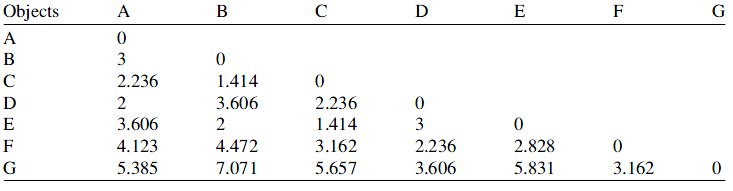
\includegraphics[scale=0.6]{images/DistanceMatrix.jpg}\\
	\end{center}
\end{figure}

\begin{itemize}
	\item In the very first step, the two
	objects exhibiting the smallest distance in the matrix are merged. Note that we
	always merge those objects with the smallest distance, regardless of the clustering
	procedure (e.g., single or complete linkage). (N.B. In the following example, ties will be broken at random.)
	\item As we can see, this happens to two
	pairs of objects, namely B and C (d(B, C) = 1.414), as well as C and E (d(C, E) =
	1.414). In the next step, we will see that it does not make any difference whether we
	first merge the one or the other, so let�s proceed by forming a new cluster, using
	objects B and C.
	\begin{figure}[h!]
		\begin{center}
			% Requires \usepackage{graphicx}
			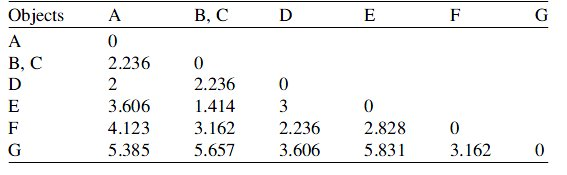
\includegraphics[scale=0.6]{images/DistanceMatrix2.jpg}\\
		\end{center}
	\end{figure}
	\item Having made this decision, we then form a new distance matrix by considering
	the single linkage decision rule as discussed above. According to this rule, the
	distance from, for example, object A to the newly formed cluster is the minimum of
	d(A, B) and d(A, C). As d(A, C) is smaller than d(A, B), the distance from A to the
	newly formed cluster is equal to d(A, C); that is, 2.236.
	\item We also compute the
	distances from cluster [B,C] (clusters are indicated by means of squared brackets)
	to all other objects (i.e. D, E, F, G) and simply copy the remaining distances � such
	as d(E, F) � that the previous clustering has not affected.
	\begin{figure}[h!]
		\begin{center}
			% Requires \usepackage{graphicx}
			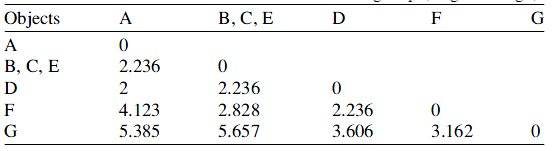
\includegraphics[scale=0.6]{images/DistanceMatrix3.jpg}\\
		\end{center}
	\end{figure}
	\item Continuing the clustering procedure, we simply repeat the last step by merging
	the objects in the new distance matrix that exhibit the smallest distance (in this case,
	the newly formed cluster [B, C] and object E) and calculate the distance from this
	cluster to all other objects.
	\begin{figure}[h!]
		\begin{center}
			% Requires \usepackage{graphicx}
			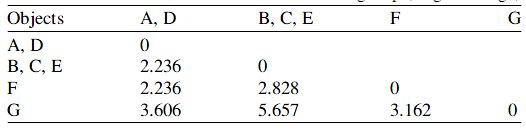
\includegraphics[scale=0.6]{images/DistanceMatrix4.jpg}\\
		\end{center}
	\end{figure}
	\item We continue in the same fashion until one cluster is left. By following the single linkage procedure, the last steps involve the merger
	of cluster [A,B,C,D,E,F] and object G at a distance of 3.162.
	\begin{figure}[h!]
		\begin{center}
			% Requires \usepackage{graphicx}
			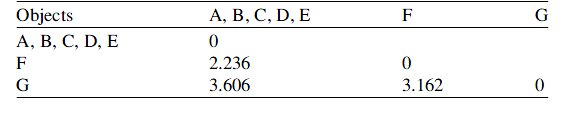
\includegraphics[scale=0.6]{images/DistanceMatrix5.jpg}\\
		\end{center}
	\end{figure}
	\begin{figure}[h!]
		\begin{center}
			% Requires \usepackage{graphicx}
			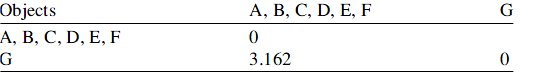
\includegraphics[scale=0.6]{images/DistanceMatrix6.jpg}\\
		\end{center}
	\end{figure}
\end{itemize}
\newpage




\section{ More on Two-Step Clustering}
\subsection{Step 1: Pre-clustering: Making Little Clusters}
The first step of the two-step procedure is formation of pre-clusters. The goal of pre-clustering is to reduce the size of the Distance matrix (the matrix that contains distances between all
possible pairs of cases). Pre-clusters are just clusters of the original cases that are used in place of the raw data in the hierarchical clustering. As a case is read, the algorithm
decides, based on a distance measure, if the current case should be merged with a previously formed pre-cluster or start a new precluster.

When preclustering is complete, all cases in the same precluster are treated as a single entity. The size of the distance matrix is no longer dependent on the number of cases but on the number of preclusters.

\subsection{Step 2: Hierarchical Clustering of Preclusters}
In the second step, SPSS uses the standard hierarchical clustering algorithm on the
preclusters. Forming clusters hierarchically lets you explore a range of solutions with
different numbers of clusters.
Tip: The Options dialog box lets you control the number of preclusters. Large numbers
of preclusters give better results because the cases are more similar in a precluster;
however, forming many preclusters slows the algorithm.

%-------------------------------------------------------------------------%
\newpage

\subsection{Step 1: Pre-clustering: Making Little Clusters}
The first step of the two-step procedure is formation of pre-clusters. The goal of pre-clustering is to reduce the size of the Distance matrix (the matrix that contains distances between all
possible pairs of cases). Pre-clusters are just clusters of the original cases that are used in place of the raw data in the hierarchical clustering. As a case is read, the algorithm
decides, based on a distance measure, if the current case should be merged with a previously formed pre-cluster or start a new precluster.

When preclustering is complete, all cases in the same precluster are treated as a single entity. The size of the distance matrix is no longer dependent on the number of cases but on the number of preclusters.

\subsection{Step 2: Hierarchical Clustering of Preclusters}
In the second step, SPSS uses the standard hierarchical clustering algorithm on the
preclusters. Forming clusters hierarchically lets you explore a range of solutions with
different numbers of clusters.
Tip: The Options dialog box lets you control the number of preclusters. Large numbers
of preclusters give better results because the cases are more similar in a precluster;
however, forming many preclusters slows the algorithm.

Some of the options you can specify when using two-step clustering are:
\textbf{Standardization:} The algorithm will automatically standardize all of the variables
unless you override this option.

\textbf{Distance measures:} If your data are a mixture of continuous and categorical variables,
you can use only the log-likelihood criterion. The distance between two clusters
depends on the decrease in the log-likelihood when they are combined into a single
cluster. If the data are only continuous variables, you can use the Euclidean
distance between two cluster centers. Depending on the distance measure selected,
cases are assigned to the cluster that leads to the largest log-likelihood or to the cluster
that has the smallest Euclidean distance.


\textbf{Number of clusters:} You can specify the number of clusters to be formed, or you can let
the algorithm select the optimal number based on either the Schwarz Bayesian
Criterion or the Akaike information criterion.


\textbf{Outlier handling:} You have the option to create a separate cluster for cases that don't fit
well into any other cluster.


\textbf{Range of solutions:} You can specify the range of cluster solutions that you want to see.

\section{Two-Step Cluster}
When you have a really large data set or you need a clustering procedure that can rapidly form clusters on the basis of either categorical or continuous data, neither of the previous two procedures are entirely appropriate. Hierarchical clustering requires a matrix of distances between all pairs of cases, and k-means requires shuffling cases in and out of clusters and knowing the number of clusters in advance.

The Two-Step Cluster Analysis procedure was designed for such applications. The name two-step clustering is already an indication that the algorithm is based on a two-stage approach: In the first stage, the algorithm undertakes a procedure that is very similar to the k-means algorithm. Based on these results, the two-step
procedure conducts a modified hierarchical agglomerative clustering procedure that
combines the objects sequentially to form homogenous clusters. This is done by
building a so-called \textbf{\textit{cluster feature tree}} whose \textbf{\textit{leaves}} represent distinct objects in the dataset. The procedure can handle categorical and continuous variables simultaneously
and offers the user the flexibility to specify the cluster numbers as well as
the maximum number of clusters, or to allow the technique to automatically choose
the number of clusters on the basis of statistical evaluation criteria.

The Two-Step Cluster Analysis requires only one pass of data
(which is important for very large data files).

Additionally, the procedure indicates each variable�s
importance for the construction of a specific cluster. These desirable features make
the somewhat less popular two-step clustering a viable alternative to the traditional
methods.
\section{Measures of Fit}
Two-Step Cluster Analysis guides the decision of how many clusters to retain from the data by
calculating measures-of-fit such as \textbf{\textit{Akaike�s Information Criterion (AIC)}} or \textbf{\textit{Bayes Information Criterion (BIC)}}.

These are relative measures of goodness-of-fit and are used to compare different
solutions with different numbers of segments.(``Relative" means that these criteria
are not scaled on a range of, for example, 0 to 1 but can generally take any value.)
Compared to an alternative solution with a different number of segments, smaller
values in AIC or BIC indicate an increased fit.

SPSS computes solutions for different
segment numbers (up to the maximum number of segments specified before) and
chooses the appropriate solution by looking for the smallest value in the chosen
criterion. However, which criterion should we choose? AIC is well-known for
overestimating the correct number of segments, while BIC has a slight tendency
to underestimate this number.

Thus, it is worthwhile comparing the clustering
outcomes of both criteria and selecting a smaller number of segments than
actually indicated by AIC. Nevertheless, when running two separate analyses,
one based on AIC and the other based on BIC, SPSS usually renders the same
results.
\subsection{AIC and BIC in Two-Step Cluster Analysis}

(Removed from Last Week's Class due to Version Update)

Two-Step Cluster Analysis guides the decision of how many clusters to retain from the data by
calculating measures-of-fit such as \textbf{\textit{Akaike�s Information Criterion (AIC)}} or \textbf{\textit{Bayes Information Criterion (BIC)}}.

These are relative measures of goodness-of-fit and are used to compare different
solutions with different numbers of segments.(``Relative" means that these criteria
are not scaled on a range of, for example, 0 to 1 but can generally take any value.)


\textbf{\textit{Important}}: Compared to an alternative solution with a different number of segments, smaller
values in AIC or BIC indicate an increased fit.

SPSS computes solutions for different segment numbers (up to the maximum number of segments specified before) and
chooses the appropriate solution by looking for the smallest value in the chosen
criterion. However, which criterion should we choose?
\begin{itemize}
	\item AIC is well-known for
	overestimating the correct number of segments
	\item BIC has a slight tendency
	to underestimate this number.
\end{itemize}

Thus, it is worthwhile comparing the clustering
outcomes of both criteria and selecting a smaller number of segments than
actually indicated by AIC. Nevertheless, when running two separate analyses,
one based on AIC and the other based on BIC, SPSS usually renders the same
results.

Once you make some choices or do nothing and go with the defaults, the clusters are
formed. At this point, you can consider whether the number of clusters is ``good". If
automated cluster selection is used, SPSS prints a table of statistics for different
numbers of clusters, an excerpt of which is shown in the figure below. You are interested
in finding the number of clusters at which the Schwarz BIC becomes small , but also the change in BIC between
adjacent number of clusters is small. 

The decision of how much benefit accrued by another cluster is very subjective. In addition to the BIC, a high ratio of distance of measures is desirable. In the figure below, the number of clusters with this highest ratio is three.

\begin{figure}[h!]
	\begin{centering}
		% Requires \usepackage{graphicx}
		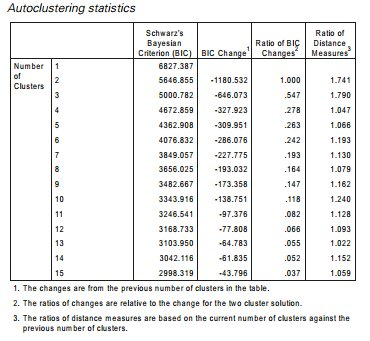
\includegraphics[width=10cm]{images/TwoStep1.jpg}\\
		\caption{Schwarz Bayesian Information Criterion}
	\end{centering}
\end{figure}


Information Criterions
We define two types of information criterion: the Akaike Information Criterion (AIC) and the
Schwarz?s Bayesian Information Criterion (BIC). The Akaike information criterion is a measure
of the relative goodness of fit of a statistical model.
AIC = 2p ? 2 ln(L)


%=================================================%
\begin{itemize}
	\item p is the number of predictor variables in the model.
	\item L is the value of the Likelihood function for the model in question.
	\item For AIC to be optimal, n must be large compared to p.
\end{itemize}

An alternative to the AIC is the Schwarz BIC, which additionally takes into account the
sample size n.
BIC = p ln n ? 2 ln(L)
When using the AIC (or BIC) for selecting the optimal model, we choose the model for which
the AIC (or BIC) value is lowest.


Akaike Information Criterion

\begin{itemize}
	\item Akaike?s information criterionis a measure of the goodness of fit of an estimated statistical
	model. The AIC was developed by Hirotsugu Akaike under the name of ?an information
	criterion? in 1971.
	\item The AIC is a model selection tool i.e. a method of comparing two or more candidate
	regression models. The AIC methodology attempts to find the model that best explains
	the data with a minimum of parameters. (i.e. in keeping with the law of parsimony)
	\item The AIC is calculated using the ?likelihood function? and the number of parameters .
	The likelihood value is generally given in code output, as a complement to the AIC.
	(Likelihood function is not on our course)
	\item Given a data set, several competing models may be ranked according to their AIC, with
	the one having the lowest AIC being the best. (Although, a difference in AIC values of
	less than two is considered negligible).
	
\end{itemize}

%=================================================%

\end{document}
%------------------------------------------------------------------------------%\end{document}


